% !TeX root = ./TMA04.tex
\newcommand{\w}{v + \epsilon \xi + \mathcal{O}\lr{\epsilon^2}}
\newcommand{\z}{\epsilon \xi + \mathcal{O}\lr{\epsilon^2}}%
\renewcommand{\ve}{v_\epsilon}%
\graphicspath{ {./images/}}%
\begin{figure}[h]
\centering
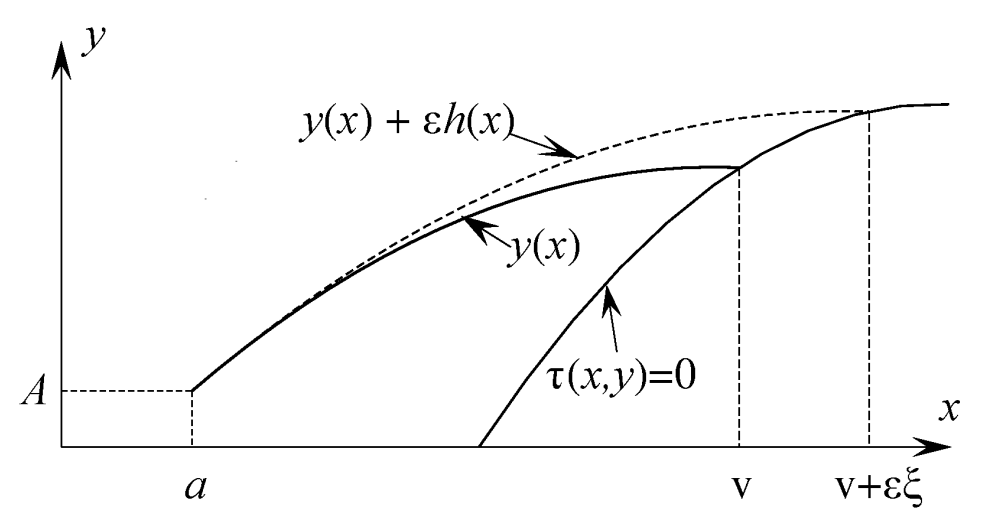
\includegraphics[width=\textwidth]{figure10_6.png}
\caption{Diagram showing the stationary path (solid line) and a varied path (dashed line) for a problem in which the left-hand end is fixed, but the other end is free to move along the line defined by $\tau(x, y) = 0$.}
\label{fig:mesh1}
\end{figure}

Given the perturbed path\marginnote{This Figure~10.6 taken from the module notes p225.}[-7cm]%
\begin{equation}
	\label{eq:4.1}
	y_\epsilon(x) = y(x) + \epsilon h(x),
\end{equation}
the Taylor series to the first-order of \eqref{eq:4.1} at point $x=v$ (see figure \ref{fig:mesh1}) is given in \eqref{eq:4.2}.\marginnote{The point $x=v$ is known as the point of expansion. HB p8.}[-0.5cm]
\begin{equation}
\begin{split}
\label{eq:4.2}
y_\epsilon(x)=\lr{y(v) + \epsilon h(v)} + \lr{y^\prime(v) + \epsilon h^\prime(v)}(x - v) + \mathcal{O}\lr{\lr{x -v}^2}.
\end{split}
\end{equation}
Now, determining the value of \eqref{eq:4.2} at $v_\epsilon = v + \epsilon \xi + \mathcal{O}\lr{\epsilon^2}$ where $v_\epsilon$ is the perturbed value of $v$:
\begin{equation*}
\begin{split}
y_\epsilon(v_\epsilon)&= y(v) + \epsilon h(v)\\ 
&\;\;+ (\cancel{v} + \epsilon \xi + \mathcal{O}\lr{\epsilon^2}\cancel{-v})\lr{y^\prime(v) +\epsilon h^\prime(v)}\\ 
&\;\;+ \mathcal{O}\lr{\lr{\cancel{v} + \epsilon \xi + \mathcal{O}\lr{\epsilon^2}\cancel{-v}}^2},\\\\
y_\epsilon(v_\epsilon)&= y(v) + \epsilon h(v)\\
&\;\;+ (\z)\lr{y^\prime(v) +\epsilon h^\prime(v)}\\
&\;\;+ \mathcal{O}\lr{\lr{\z}^2},
\end{split}
\end{equation*}
\begin{equation*}
\begin{split}
y_\epsilon(v_\epsilon)&= y(v) + \epsilon h(v)\\
&\;\;+ \epsilon\xi\lr{y^\prime(v) +\epsilon h^\prime(v)}\\
&\;\;+ \mathcal{O}\lr{\epsilon^2}\lr{y^\prime(v) +\epsilon h^\prime(v)}\\
&\;\;+ \mathcal{O}\lr{\lr{\z}^2},\\\\
y_\epsilon(v_\epsilon)&=y(v) + \epsilon \lr{h(v) + \xi y^\prime(v)}\\
&\;\;+ \underbrace{\epsilon^2\xi h^\prime(v)
+ \mathcal{O} \lr{\epsilon^2}\lr{y^\prime(v) +\epsilon h^\prime(v)}+ \mathcal{O}\lr{\lr{\z}^2}}_\text{These are all second-order terms in $\epsilon$.}.
\end{split}
\end{equation*}
Thus,
\begin{equation}
\label{eq:4.3}
\begin{split}
y_\epsilon(v_\epsilon)&=y(v) + \epsilon \lr{h(v) + \xi y^\prime(v)} + \mathcal{O}\lr{\epsilon^2},
\end{split}
\end{equation}
as required.

To show that at $(x,y) = (v,y(v))$,
\[\xi\lr{\tau_x+y^\prime(v)\tau_y}+h(v)\tau_y=0\]
the 2D Taylor expansion to the first-order of $\tau(x,y)$ at point $x=a, y=b$ is required, namely,
\begin{equation}
\label{eq:4.4}
\tau(x,y) = \tau(a,b) + \tau_x(a,b)\lrs{x-a} + \tau_y(a,b)\lrs{y-b}.
\end{equation}
Evaluating \eqref{eq:4.4} with $x=v_\epsilon = v + \epsilon\xi$ and $y=y_\epsilon(v_\epsilon)=y(v) + \epsilon\lr{y^\prime(v)\xi+h(v)}$ gives,
\begin{equation*}
\begin{split}
\tau&\lr{\ve,y_\epsilon(\ve)} = \tau(v+\epsilon\xi,y(v)+\epsilon\lr{y^\prime(v)\xi+h(v)}\\
&\;\;= \cancelto{0}{\tau\lr{v,y(v)}} + \tau_x\lr{v,y(v)}\lrs{\ve-v}+\tau_y\lr{v,y(v)}\lrs{y_\epsilon(\ve)-y(v)},\\
&\;\;= \tau_x\lr{v,y(v)}\lrs{\ve-v}+\tau_y\lr{v,y(v)}\lrs{y_\epsilon(\ve)-y(v)},\\
&\;\;= \tau_x\lr{v,y(v)}\lrs{\cancel{v}+\epsilon\xi\cancel{-v}}+\tau_y\lr{v,y(v)}\lrs{\cancel{y(v)} + \epsilon\lr{y^\prime(v)\xi+h(v)}\cancel{-y(v)}},\\
&\;\;= \tau_x\lr{v,y(v)}\epsilon\xi+\tau_y\lr{v,y(v)}\epsilon\lr{y^\prime(v)\xi+h(v)},\\
&\;\;= \epsilon\lrs{\tau_x\lr{v,y(v)}\xi+\tau_y\lr{v,y(v)}\lr{y^\prime(v)\xi+h(v)}},\\
\end{split}
\end{equation*}
Recall that $\tau\lr{\ve,y_\epsilon(\ve)} = 0$ and therefore,
\begin{equation*}
\begin{split}
	\epsilon\lrs{\tau_x\lr{v,y(v)}\xi+\tau_y\lr{v,y(v)}\lr{y^\prime(v)\xi+h(v)}} &= 0,\\
	\tau_x\lr{v,y(v)}\xi+\tau_y\lr{v,y(v)}\lr{y^\prime(v)\xi+h(v)} &= 0,\\
\end{split}
\end{equation*}
\begin{equation}
	\label{eq:4.5}
	\xi\lrs{\tau_x\lr{v,y(v)} + \tau_y\lr{v,y(v)} y^\prime(v)} + \tau_y\lr{v,y(v)} h(v) = 0,
\end{equation}
as required.

